%%%%%%%%%%%%%%%%%%%%%%%%%%%%%%%%%%%%%%%%%%%%%%%%%%%%%%%%%%%%%%%%%%
%  Thesis template file  prepared by:
%  Thyge Knüppel, tkn@elektro.dtu.dk, DTU Elektro, May 2008
%  Based on the work of Jan Larsen, IMM, DTU (cf. http://www2.imm.dtu.dk/teaching/phd/)
%
%  CET June 2010 edited Charlotte K. Madsen
%%%%%%%%%%%%%%%%%%%%%%%%%%%%%%%%%%%%%%%%%%%%%%%%%%%%%%%%%%%%%%%%%%

%%%%%% Compilation: 
% compilation using latex (i.e. via a ps file)
\documentclass[a4paper,11pt,oneside,openright,dvips]{book}

% compilation using PDFLATEX - Note that pdflatex is known to have issues with
% some of the pstricks-packages
% 	\documentclass[a4paper,11pt,twoside,openright,pdftex]{book}
%%%%%%%%%%%%%%%%%%%%%%%%%%%%%%%%%%%%%%%%%%

%%%%%%%%%%%%%%%%%%%%%%%%%%%%%%%%%%%%%%%%%%%%%%%%%%%%%%%%%%%%%%%%%%
% Input information for cover, titlepages:
% Sould be EDITED to match your work!

%multiple authors separated by "\\"
%If there are multiple authors adjust the \vspace 
%in thesislayout.sty as necessary 
\def\ThesisAuthor{Mads Lundt, s103439 \\
			      Matthias Larsen, s103437 \\
			      Joachim Jensen, s103430}
			      
%list of authors for pdf
%properties. Multiple authors separated by ","
\def\ThesisAuthorForHyperref{Mads Lundt, s103439 , Matthias Larsen, s103437 , Joachim Jensen, s103430}

%project title
\def\ThesisTitle{Weather data visualization}

%subtitle - if any
\def\Subtitle{A Graphical User Interface (GUI) for weather radar and wind energy data visualization and analysis} 

%keywords for the pdf file
\def\thesiskeywords{Software Technology Project, Weather data visualization} 

%only for pdf properties - doesn't appear on printed versions
\def\thesissubject{}

%list of supervisors. multiple supervisors are separated by "\\"
\def\Supervisor{Pierre Pinson//Pierre-Julien Trombe} 

%type of project (see README file %for explanation)
\def\projecttype{Software Technology Project, June 2012} 

%type \ISBNNUMBER{ISBN: xxx} if your project has one
\def\ISBNNUMBER{} 

%date of publication
\def\DatePublished{June, 2012} 

%project class (see README file for explanation)
\def\Klasse{1 (public)} 

%obtained degree (see README file for explanation)
\def\Degree{Master of Science in Engineering (M.Sc.Eng.)} 

%# of ECTS points 
\def\ECTSpoints{10} 

%edition
\def\Udgave{First} 

 %name of copyright and year
\def\Owner{Mads Lundt, Matthias Larsen, Joachim Jensen, 2012}
%%%%%%%%%%%%%%%%%%%%%%%%%%%%%%%%%%%%%%%%%%%%%%%%%%%%%%%%%%%%%%%%%%

%%%%%%%%%%%%%%%%%%%%%%%%%%%%%%%%%%%%%%%%%%%%%%%%%%%%%%%%%%%%%%%%%%
%%%%%%%%%%%%% Change settings: (compile twice )%%%%%%%%%%%%%%%%%%%%%%
%OBS: choose this for final version (official set of title pages) 
\def\thesisversion{final} 
%OBS: choose this for working-copy draft version (simple title page and no info page)
%\def\thesisversion{workingcopy} 
%OBS: choose this for draft version (offical title pages, no info page and water marked)
%\def\thesisversion{draft} 
%OBS: choose this for draft version (simple title page /w logo)
%\def\thesisversion{majorassignment}
%OBS: choose this for draft version (only simple title page /w logo)
%\def\thesisversion{minorassignement}  
                         

%\def\thesislinks{no}%OBS: choose this for paper version (no colored links) 
\def\thesislinks{yes}%OBS: choose this for online version (with links)
%%%%%%%%%%%%%%%%%%%%%%%%%%%%%%%%%%%%%%%%%%%%%%%%%%%%%%%%%%%%%%%%%%

%%%  For changing language: (compile twice -first time gives errors)%%%
\def\thesislanguage{en} %OBS: compile document for English 
%\def\thesislanguage{da}  %OBS:  compile document for Danish


%%%%%%%%%%%%%%%%%%%%%%%%%%%%%%%%%%%%%%%%%%
% Load style definitions, packages, etc:
	\usepackage{style/thesisdef} 		% packages  listings aso
	\usepackage{style/thesislayout} 	% layout; headings, pagemargin, theorems aso
	\usepackage{style/mathboxes}		% example and other math boxes
	\usepackage{style/Mythesis} 	  	% Locals editings to only your thesis
%%%%%%%%%%%%%%%%%%%%%%%%%%%%%%%%%%%%%%%%%%
% END of premable
%%%%%%%%%%%%%%%%%%%%%%%%%%%%%%%%%%%%%%%%%%%%%%%%%%%%%%%%%%%%%%%%%%

%%%%%%%%%%%%%%%%%%%%%%%%%%%% DOCUMENT %%%%%%%%%%%%%%%%%%%%%%%%%%%%
	\begin{document}

%%%%%%%%%%%%%%%%% Edit ONLY for printing type:
% Front matter:
	\frontmatter

  \ifx\thesisversion\printversion
	% for final version include standard dtu cover pages
	\pagenumbering{alph}%dummy numbering for pdf-file (numbering set as a
                    %pdf-property and is NOT visible on the document). The
                    %hyperref package complains if duplicate numbering exists
	\coverpages    %generates the first four pages (thesislayout.sty)
	\else
%for draft version use simple title page:
	\title{\ThesisTitle{} - \Subtitle{}}
	\author{\ThesisAuthor}
	\thispagestyle{empty}
	\maketitle
	\clearpage{\thispagestyle{empty}\cleardoublepage}
   \fi
%%%%%%%%%%%%%%%%%%%%%%%%%%%%%%%%%%%%%%%%%%

%%%%%%%%%%%%%%%%%%%%%%%%%%%%%%%%%%%%%%%%%%%%%%%%%%%%%%%%%%%%%%%%%%
% PREFACE CHAPTERS INCLUDE: files are in folder "file"
	%\pagestyle{empty} 	%For first few pages %\markboth{}{}
	
%% Ad to List of Contents:
\chapter*{Acknowledgements}
%The solutions provided by this report to the Weather data visualization -- A Graphical User Interface (GUI) for weather radar and wind energy data visualization and analysis, has been developed by Mads Lundt ($s103439$), Matthias Larsen ($s103437$) and Joachim Jensen ($s103430$).

We would like to express our gratitude to Pierre Pinson and Pierre-Julien Trombe for giving us the opportunity to work on this project.

Morten H. S. Jespersen for his assistance in the layout of the paper.

Especially, we would like to give a special thanks to Adam L. Baxter for proofreading this paper.
	
\pagenumbering{roman}
  \ifx\thesisversion\printversion % no resumes in draft-version
%% Ad to List of Contents:
\chapter*{Abstract, Resumé}
	\ifx\thesislanguage\danishlang
	\addcontentsline{toc}{chapter}{Resumé}
	\else
	\addcontentsline{toc}{chapter}{Abstract}
	\fi
% State the problem, your approach and solution, and the main contributions of the paper. Include little if any background and motivation. Be factual but comprehensive. The material in the abstract should not be repeated later word for word in the paper.
Data for weather analysis and forecasts consists of enormous amounts of data.

To predict the weather, a lot of variables is in play including wind speed, pressure and tendency.

Comparing huge amounts of data quickly becomes hard. Most people interprets images easier than numbers, hence the need for some sort of visualization for the data sets.

Today no free application exists for visualizing the weather data except for two earlier attempts: one in MATLAB and one with Google Maps. These earlier application were not flexible enough to be used in bigger context.

This report shows the development and considerations throughout the project of an application that might serve as the beginning of a new common open source platform for analyzing, visualizing and comparing weather related data.
\todo[inline]{Abstract / Resume}
\fi
%% Ad to List of Contents:
%\chapter*{Resumé, Abstract}
%	\ifx\thesislanguage\danishlang
%	\addcontentsline{toc}{chapter}{Abstract}
%	\else
%	\addcontentsline{toc}{chapter}{Resumé}
%	\fi
%\input{file/resume}
%  \fi
% if a chapter is wanted BEFORE lists
%% Ad to List of Contents:
%\chapter*{Preface, Forord}
%	\ifx\thesislanguage\danishlang
%	\addcontentsline{toc}{chapter}{Forord}
%	\else
%	\addcontentsline{toc}{chapter}{Preface}
%	\fi
%\input{file/preface} %lines above can be moved into this file
%%%%%%%%%%%%%%%%%%%%%%%%%%%%%%%%%%%%%%%%%%%%%%%%%%%%%%%%%%%%%%%%%%

%%%%%%%%%%%%%%%%%%%%%%%%%%%%%%%%%%%%%%%%%%
% TOC,LOF,LOT and SETUP HEADER: (should not be edited)
	%\pagestyle{fancyplain}		%'plain' enable center-food-pagenumber only
							%'fancyplain' gives right-left numbers

	\cleardoublepage 	\phantomsection  	% makes pdf-hyperref work in adobe
	\ifx\thesislanguage\danishlang
	\addcontentsline{toc}{chapter}{Indhold}
	\else
	\addcontentsline{toc}{chapter}{Contents}
	\fi
\tableofcontents  

  \ifx\thesisversion\printversion	
	\cleardoublepage 	\phantomsection  	% makes pdf-hyperref work in adobe
	\ifx\thesislanguage\danishlang
	\addcontentsline{toc}{chapter}{Figurliste}
	\else
	\addcontentsline{toc}{chapter}{List of Figures}
	\fi
\listoffigures

	\cleardoublepage 	\phantomsection  	% makes pdf-hyperref work in adobe
	\ifx\thesislanguage\danishlang
	\addcontentsline{toc}{chapter}{Tabelliste}
	\else
	\addcontentsline{toc}{chapter}{List of Tables}
	\fi
\listoftables
  
  	\cleardoublepage 	\phantomsection  	% makes pdf-hyperref work in adobe
	\ifx\thesislanguage\danishlang
	\addcontentsline{toc}{chapter}{Kildekode liste}
	\else
	\addcontentsline{toc}{chapter}{List of Source code}
	\fi
\lstlistoflistings
  \fi
%%%%%%%%%%%%%%%%%%%%%%%%%%%%%%%%%%%%%%%%%%

\label{fancy:frontend} %for 'of page /x'
\clearpage{\thispagestyle{empty}\cleardoublepage}

%%%%%%%%%%%%%%%%%%%%%%%%%%%%%%%%%%%%%%%%%%%%%%%%%%%%%%%%%%%%%%%%%%
% MAIN CHAPTERS INCLUDED FROM FOLDER  "file":
	\mainmatter %\setcounter{page}{1}\pagenumbering{arabic} if mainmatter fails

% if a chapter is wanted after lists or other unnumbered chapter
%% Ad to List of Contents (can also be the first entry after \chapter in the file:
	\cleardoublepage 	\phantomsection  	
	\ifx\thesislanguage\danishlang
	%\addcontentsline{toc}{chapter}{Introduktion}
	\markboth{Forord}{}
	\else
	%\addcontentsline{toc}{chapter}{Introduction}
	\markboth{Preface}{}
	\fi
\chapter{Introduction}
\label{sec:introduction}

% The Introduction is crucially important. By the time a referee has finished the Introduction, he's probably made an initial decision about whether to accept or reject the paper -- he'll read the rest of the paper looking for evidence to support his decision. A casual reader will continue on if the Introduction captivated him, and will set the paper aside otherwise. Again, the Introduction is crucially important.

% Here is the Stanford InfoLab's patented five-point structure for Introductions. Unless there's a good argument against it, the Introduction should consist of five paragraphs answering the following five questions:

% What is the problem?
The problem with this project is analysing the different kinds of data and visualize it in a smooth and easy way. There are other weather applications on the market, but one of the requirements to create the new weather application, is using open source (OpenStreetMap, Qt etc.). We had different kinds of data in different languages, CSV-files, WRK-files and NC-files. We only did the implementation for CSV-files and WRK-files.\\
We are very focused on getting high performance and getting this optimized - that was one of the biggest challenges.

% Why is it interesting and important?
This is interesting because there is a lot of data to analyse and visualize, and still want\todo[fancyline,color=green]{Adam: Mangler et subjekt} high performance and user-friendly overview. There have been combined different programming language to get it optimized. All this and still it should be functional and user-friendly.

% Why is it hard? (E.g., why do naive approaches fail?)
This is tough, because there had to be some changes during its construction, such as implement database integration, to get this optimized. Many of these changes are to satisfy our own requirements through the project.\\
There are a lot of data to analyse and visualize, so there has be figured out how to do this in the best possible way.

% Why hasn't it been solved before? (Or, what's wrong with previous proposed solutions? How does mine differ?)
There are other applications out there, like DMI and TV2-vejret, but none of these satisfied our requirements that was specified at the beginning. DMI had many different data, but wasn't created in a user-friendly way and TV2-vejret only have weather forecast. There are similar weather programs out there, but none of these have either user-friendly way of handling huge amount data or using open source.

% What are the key components of my approach and results? Also include any specific limitations.
\todo[inline]{What are the key components of my approach and results? Also include any specific limitations?}

% Then have a final paragraph or subsection: "Summary of Contributions". It should list the major contributions in bullet form, mentioning in which sections they can be found. This material doubles as an outline of the rest of the paper, saving space and eliminating redundancy.
\chapter{Related work}
A GUI has been developed in Matlab..

A second attempt made use of Google Maps..
\chapter{Body}
\section{The use of frameworks}
Using frameworks because of the decreased development time due to already developed and tested libraries for various tasks such as database accesss, file handling and file uploading.

\section{The C++ application}
\subsection{Why a C++ application?}
We're using a C++ application because it is much faster to parse huge files in C++ than PHP or JavaScript.
The choice of language was because we had some knowledge of both C and C++. C++ is object oriented where as C is procedural language, and seeing as we all favour object oriented programming, the choice between the two was easy.

We could have chosen other languages such as F, F\#, Java, Perl or Ruby, but our limited knowledge about these made us stick with C++, which is also quite fast and portable.

\subsection{Why Qt?}
We've decided to use Qt because of the support and community around it. It's very mature and most importantly, object oriented.

\subsection{Return codes}
The C++ application returns the following codes to the PHP after processing data:
\begin{table}[htbp]
\centering
\begin{tabular}{|l|l|}
\hline
\textbf{Code} & \textbf{Explanation}\\
\hline
0 & Failure\\
\hline
1 & Success\\
\hline
2 & Success, unkown params ignored\\
\hline
10 & Failed, missing fileid\\
\hline
11 & Failed, missing filename\\
\hline
12 & Failed, missing type\\
\hline
20 & Unknown file type\\
\hline
21 & File not found\\
\hline
22 & Invalid file, or wrongly formatted\\
\hline
30 & Could not read input file\\
\hline
31 & Could not write to input file\\
\hline
32 & Could not read output file\\
\hline
33 & Could not write to output file\\
\hline
34 & Could not delete output file\\
\hline
\end{tabular}
\label{tab:cppReturnCodes}
\caption{Return codes from the C++ application}
\end{table}

\subsection{Extensibility}
The application is coded with extensibility in mind, and all parsers is therefore extending the base class \emph{Parser}.
The \emph{Parser} class contains the basic methods of setting the filename, opening for read and write and closing the open file handle.

\section{The PHP site}
\subsection{Why PHP?}

\subsection{Why FuelPHP?}

\subsection{Speed optimizations}
At the beginning the chart had monthly, weekly and daily view, but when loading all data for one month, the performance were so poor. This was fixed by changing views to 2-weekly, weekly and daily view.
\subsubsection{Caching}
Caching has been implemented both server and client side, to allow for maximum performance when viewing charts and radar image animations.

\begin{table}[htbp]
\centering
\begin{tabular}{|l|l|l|l|}
\hline
\textbf{Area} & \textbf{Before} & \textbf{Server side} & \textbf{Server + client side}\\
\hline
Radar & \textasciitilde 130-150 ms & \textasciitilde 35 ms & \textasciitilde 2 ms\\
\hline
Chart & \textasciitilde 300 ms & \textasciitilde 40 ms & \textasciitilde 2 ms\\
\hline
\end{tabular}
\label{tab:cppReturnCodes}
\caption{Cache benchmarks}
\end{table}

When a radar image or chart data is requested, the server checks if a cache of the output exists. If it does, it checks if the browser already have a copy of the same cache file and send a \textsf{301 Not Modified} response to the browser, telling it to its own file.
If the browser does not have a cache, or it is too old, the server sends the contents of the new cache to the browser.
If no cache is found on the server, or it has expired, the server retrieves the needed info from the database, generate the image or data to output, saves it to the cache and sends it to the browser.


\subsection{The data}
The application support the upload of the following file types:
\begin{description}
\item[csv] Observations form a wind farm. The definition can be found in appendix \ref{ap:csv}.
\item[wrk] Weather image from a radar. The file most obey the new VRIS format. See \cite{VRIS} for the definition of VRIS.
\item[zip] All supported file formats can be zipped to easily upload multiple files at the same time. Unlimited zip and folder nesting is supported\footnote{Note that there might be a limit on the file- or foldername length set by the operating system.}.
\end{description}

\section{Cross-platform compability}
The use of PHP, C++ and MySQL allows the execution of the application on almost all platforms, because the technologies used are open source and available on most platforms.

We have, however, chosen to drop support for all version of Internet Explorer, because this would increase development time drastically -- time we did not have.
\chapter{Considerations}
Through the project we had some considerations:
\begin{itemize}
\item Comparing wind farms.
\item List WRK-files in a smart way.
\item File types
\item Radar visualization
\item From and To interval
\item Map design
\item Chart design
\item Windmill icons
\end{itemize}
We were thinking about comparing wind farms, so the client should be able to open more wind farms in different pop ups. The final product only supports one pop up, because it would quickly become confusing.\\
Listing WRK-files in a smart way, like list WRK-files in daily view instead of listing them for every 10th minutes. This wasn't implemented, since we would like the user to have more control, so instead of deleting a file for the whole day, the user can delete files for every 10th minute.\\
We started with the CSV-files for wind farms, since the data was easy to read. After that, we tried WRK-files, which was a little more advanced.\\
We couldn't find a nice way to show radar names for the radar on the map. We thought about having names at the top or bottom of the radar, but it wasn't good when multiple radars very overlapping each other.\\
We wanted to have two text fields on the map - from and to - so the users could choose an interval. We replaced this with just one text field - From - because we found the second text field inappropriate.\\
Radar buttons for play, pause and reset is also inappropriate, since we have added gestures for it. If you would like to play/pause radar just press on it or to reset the radar, simply just double click on it. This make it a lot easier for the user to control the radar.\\
We had multiple design suggestions for map and chart design. At the beginning we had a scroll-in/out sidebar, which could be show/hidden. This quickly became annoying, so it was replaced by a top bar. It was important that the menu could stay hidden or didn't cover up to much of the map.\\
We wanted to have windmill icons for wind farms on the map. These were very difficult to find on the internet, so we tried to created one by our self in Photoshop. One of the problems were to get a windmill that could be seen on the very bright map. We went back to use an old windmill icon.\\

\subsection{Comparison}
It's been discussed if it should be possible to compare data from multiple wind farms at the same time, and how it should be done if that was the case.

One of the ideas was to let single click on a windmill put it in a `selected' state and a double click on a windmill would trigger the comparison view between all the windmills in the `selected' state.

The comparison view was also discussed to be either one chart, like the one implemented, but with all the data represented with different colors for each wind farm.
Another way of viewing them was to have multiple small draggable windows, each one representing a wind farm. This would allow browsing the data for each wind farm independent of each other, but also make it annoying when wanting to compare the same time and having to manually move forth or back in time on each window.

We chose to drop comparison because we fell short of time, but the above ideas could be used to develop some sort of comparison of data from multiple sources at the same time.

\chapter{Map choice}
We considered two options in the selection of map - Openstreetmap and Google maps. We have tried using Google maps on Google, Facebook, etc.. The second attempt of a weather application were using Google maps, so at the beginning we were thinking about using Google maps.

After reading about the two maps, it became Openstreetmap. We did this partly because of Google wants money if the map is used for commercial purposes. This wasn't the way we were thinking about open source.

Openstreetmap wasn't that difficult to work with, due to the well documentation from leaflet\footnote{Documentations for Openstreetmap - http://leaflet.cloudmade.com}.
\chapter{Requirements}
We stated some requirements to the final product, that should be fulfilled. 
The requirements:
\begin{itemize}
\item Web based software using opensource software.
\item Upload data to server in seperate files and compressed files.
\item Analyse and read data from CSV, WRK and NC-files.
\item Visualize the data in a nice user-friendly way.
\item Several performance requirements
\end{itemize}
We created the web based software using opensource.\\
It is allowed to upload CSV, WRK and zip-files.\\
We didn't do the implementation for the NC-files, because of difficulty and time pressure. However, CSV and WRK-files are working just fine, even if they both are compressed into one zip-file.\\
The visualizing of data are done in very user-friendly and cool design. We used a lot javascript, to create this cool and user-friendly design.\\
The performance is very good and the server is doing the most work, so even computers with poor specifications can access. We have done some caching\footnote{A collection of data duplicating original values stored on the server or by the client's web browser}, to get better performance too.\\

\section{Application requirements}
\label{sec:application_requirements}
The application requires a few things in order to run.
\begin{description}
\item[Web server] A web server is needed in order to run the web site. It is also required to have permissions to run executables. The included data parser is compiled for Windows, OSX and Ubuntu. If the web server is not allowed to run the included executables, they should be ran as a CGI script - This has not been tested however.
\item[PHP] The web server should support PHP version 5.3+.
\item[GD] The application uses GD 2.0.1+ (2.0.28+ is recommended) to create radar images.
\item[MySQL] FuelPHP supports multiple databases through drivers, but in order to support time zones correctly, we've chosen to take advantage of MySQLs own methods. This means that MySQL 5.5.20+ is required.
\item[Zoneinfo] MySQL needs Zoneinfo in order for the time zones to work properly\footnote{On linux, the following command can be executed in the terminal to import zoneinfo: \mbox{\textsf{> mysql\_tzinfo\_to\_sql /usr/share/zoneinfo | mysql -u root -p mysql}}. Other operating systems might not have the zoneinfo, and will have to download it from \url{http://dev.mysql.com/downloads/timezones.html} and import it to the mysql database.}
\item[Safe mode] Safe mode might need to be disabled in the PHP configuration, if \textsc{fopen}\footnote{See \url{http://php.net/manual/en/function.fopen.php}.} is not allowed to access some files.
\end{description}
\chapter{Smartphones}
Today many people keep them updated on the fly and to give them the opportunity, we have tried to create a design that also works on smartphones, that have smaller screens and lesser processing power. Most of the calculating is done on the server, so the requirements for client-side is almost nothing, other than showing the data that the server has performed.\\
The only problem with smartphone is the smaller screen, sometimes it can be difficult to get a good look, specially the charts are a problem.
\chapter{Work flow \& distribution}
At the beginning Dropbox\footnote{A web based file hosting service - see \cite{Dropbox}} was used to sharing files between group members, using a shared folder, all members could read and write to. It was fine at the beginning, but later when there became file conflicts , it started to get a little problematic, since Dropbox doesn't have a smart merging algorithm.
There was created a public repository at Git\footnote{A web based hosting service - see \cite{Git}} to push and pull data to the git server, so files could be changed without to many conflicts. Git was used, because of the merging algorithm and easy to use.

Git allows you to view older files and list commits\footnote{Every time a person push data to Git, he also gives a comment of what he has done. In that way it is easier to get an overview of changes.} from users through the whole project.

Git also allow other users to look at the program and and test it by them self, so it is accessible for all.

Since Git is used, everyone can access the repository\footnote{Repository \url{http://github.com/connors511/WeatherDataVisualization}} by them self. Users can't change or commit data, but can download the application and give comments to the project.

\section{Distribution}
As this software project have been carried out by a group, we have been working together as a team with constructive criticism of each other, spelling and syntax correction ect. This means that everyone have more or less had a hand in every part of the software. However:

Mads Lundt have had the main responsibility of the following parts of the software:
\begin{itemize}
\item Map (HTML + JavaScript)
\end{itemize}

Matthias Larsen have had the main responsibility of the following parts of the software:
\begin{itemize}
\item Data Parser (C++)
\end{itemize}

Joachim Jensen have had the main responsibility of the following parts of the software:
\begin{itemize}
\item File upload (PHP)
\end{itemize}
\chapter{Conclusion}
There was created a weather application, that met the requirements we stated at the beginning.
It was not easy, since there are no applications with our specified requirements, that could inspire us.

The implementation of different file types, data visualizing and database integration, to make it easier and to get higher performance, are completed in that way it was required from the beginning. While there is a lot of focus on extensibility and simplicity.
 
The implementation that did not finish, were the NC-files, due the troubles with CSV and WRK. This and coordinates converting were not implemented, due there was no test data with other coordinates, but as earlier stated, this can be implemented.

The use of Git was much better than Dropbox, that was used in the beginning, and allowed all group members to change files without too much concern for conflicts.

The final product ended up being a satisfied solution for a weather application, that could analyze and visualize the enormous amounts of data in an intuitive way.
\chapter{Future work}

Besides fixing the currently known bugs stated in BUGS REFERENCE, we have some ideas for the application, some of which have been described in ANALYSE REFERENCE that did not make it to the existing application.

\section{GPS coordinates}
There are several ways to locate positions on a map. We have used \emph{conjugate graticule}\footnote{Latitude/Longitude also known as conjugate graticule}, because the test data we had available used this. We haven't implemented for other GPS coordinates than latitude and longitude, because of the time pressure.

We know that there are other methods to get GPS coordinates - one of them is \emph{Degrees, Minutes, Seconds}. In a circle there are 360 degrees, so to get a minute each degree is split up into 60 parts, \nicefrac{1}{60}th of a degree. To get seconds each minute is split up into 60 parts, \nicefrac{1}{60}th of a minute.

To convert \emph{Degrees, Minutes, Seconds} into latitude and longitude, just simply use the formula:
\begin{equation}
Degrees~ + \left(Minutes~ \cdot \nicefrac{1}{60}\right) + \left(Seconds~ \cdot \nicefrac{1}{60} \cdot \nicefrac{1}{60}\right)
\end{equation}

Converting the other way around should be a bit more difficult, but since openstreetmap is using latitude and longitude, this isn't necessary.
\section{API}
The application has a small API\footnote{Application programming interface} that the application it self uses to retrieve some of the data.

\subsection{Radars}
A list of images for a radar can be retrieved by calling
\begin{lstlisting}[language=sh]
GET http://WEBROOT/rest/radar/list.TYPE?lat=LAT&lng=LNG&f=FROM
\end{lstlisting}
Where \textsf{WEBROOT} is the domain name of the server, \text{TYPE} is the return type\footnote{All formats supported by FuelPHPs REST controller is supported. A list of supported formats can be found at \url{http://docs.fuelphp.com/general/controllers/rest.html\#/formats}.\label{fn:fuel_rest}}, \textsf{LAT} is the latitude of the radar, \textsf{LNG} is the longitude of the radar and \text{FROM} is a date from which the data should start from.

The returned data is in array format, where each element is an array consisting of two elements. The first is the timestamp of the image, and the second is the url of the radar image relative to the \textsf{WEBROOT}.

\subsection{Wind farms}
A list of data from a given wind farm can be retrieved by calling
\begin{lstlisting}[language=sh]
GET http://WEBROOT/rest/csv/list.TYPE?id=ID&c=COL&f=FROM&t=TO
\end{lstlisting}
Where \textsf{WEBROOT} is the domain name of the server, \textsf{TYPE} is the return type\footref{fn:fuel_rest}, \textsf{ID} is ID of the wind farm, \textsf{COL} is the column\footnote{Currently \textsf{PossiblePower}, \textsf{OutputPower}, \textsf{WindSpeed}, \textsf{RegimePossible} and \textsf{OutputRegime}. Note that the columns are case-sensitive.} to fetch data from, \text{FROM} is a date from which the data should start from and \text{TO} is a date at which the data stops at.

The returned data is in array format, where each element is an array consisting of two elements. The first is the timestamp of the image, and the second is the url of the radar image relative to the \textsf{WEBROOT}.

\subsection{Jobs}
A number of files currently in queue to be parsed can be retrieved by calling
\begin{lstlisting}[language=sh]
GET http://WEBROOT/rest/jobs/list.TYPE
\end{lstlisting}
Where \textsf{WEBROOT} is the domain name of the server.

\subsection{Upload}
It is possible to send data to the application, just as if they were being uploaded manually. This allows for remote services to send `real time' data to the application. To send data to the server, the following call should be made:
\begin{lstlisting}[language=sh]
curl -F "path=@FILE" http://WEBROOT/api/upload -H "X-KEY: KEY=" -H "X-TIMEZONE: ZONE" -X POST
\end{lstlisting}
Where \textsf{FILE} is the path to the file on the senders machine, \textsf{WEBROOT} is the domain name of the server, \textsf{KEY} is an API key and \textsf{ZONE} is the time zone given by MySQLs Zoneinfo\footnote{See section \ref{sec:application_requirements} for notes about installation of Zoneinfo}.

An example call, to upload \textsf{ekxr20101218\_2350.wrk} with UTC timestamps to the \textsf{WEBROOT} server with the default admin user woudl look like this:
\begin{lstlisting}[language=sh]
curl -F "path=@ekxr20101218_2350.wrk" http://WEBROOT/api/upload -H "X-KEY: YWqmPGH+dOEvOh6pf83a62lzJ1QQLHRMPHhNIaohB3s=" -H "X-TIMEZONE: UTC" -X POST
\end{lstlisting}
\chapter{Design}
There have been several design ideas. Many changes through the project and many considerations.
\section{Map}
At the beginning we had a sidebar which could be visible or hidden. Later we found out that there is no need for a big menu, so we removed the sidebar and added a tiny top bar, with only the necessary options.

First mockup:
\begin{figure}[htbp]
   \centering
   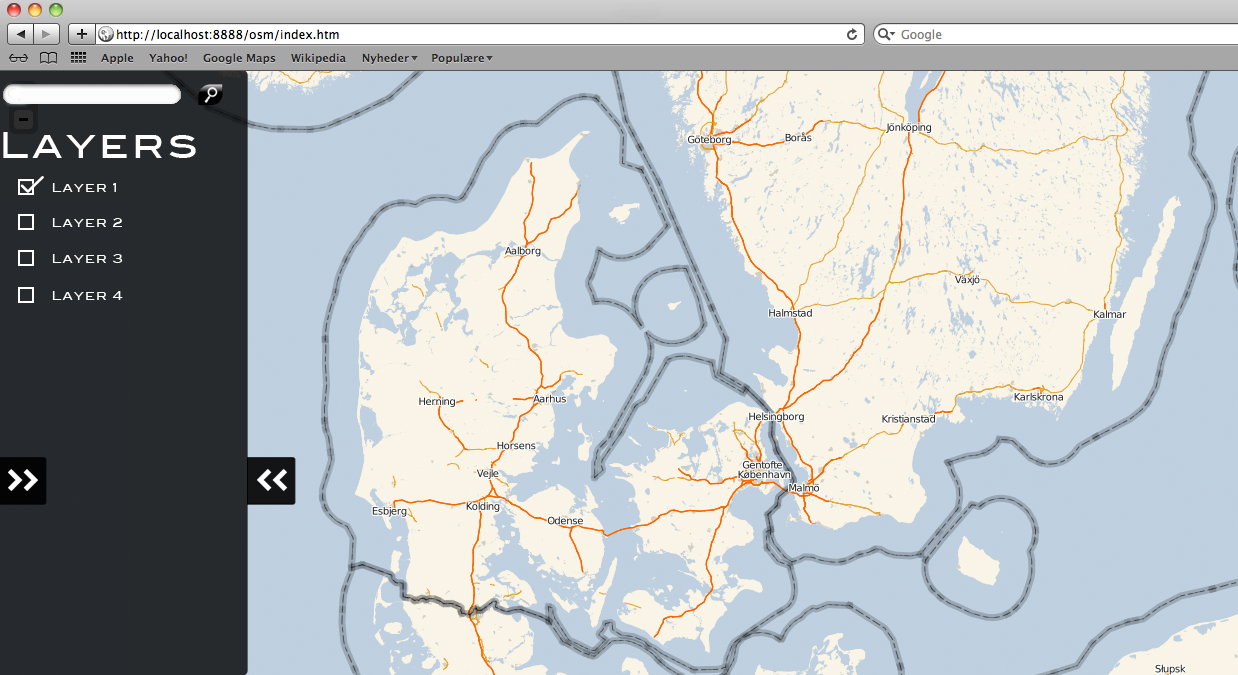
\includegraphics[scale=.3]{figure/design_map_v1.eps}
   \caption{Map - version 1}
\end{figure}

We would like to have different layers on the map at the beginning, but this was unnecessary, so it was quickly removed.

Now we have created a cool design which is easy to get used to and all relevant informations can be accessed easily and without to much clicking.
There have also been added some gestures to control the radar easily.\\
The top bar has a date field to know which date the radar should get data from. This date will be transferred to the chart window, also.

\begin{figure}[htbp]
   \centering
   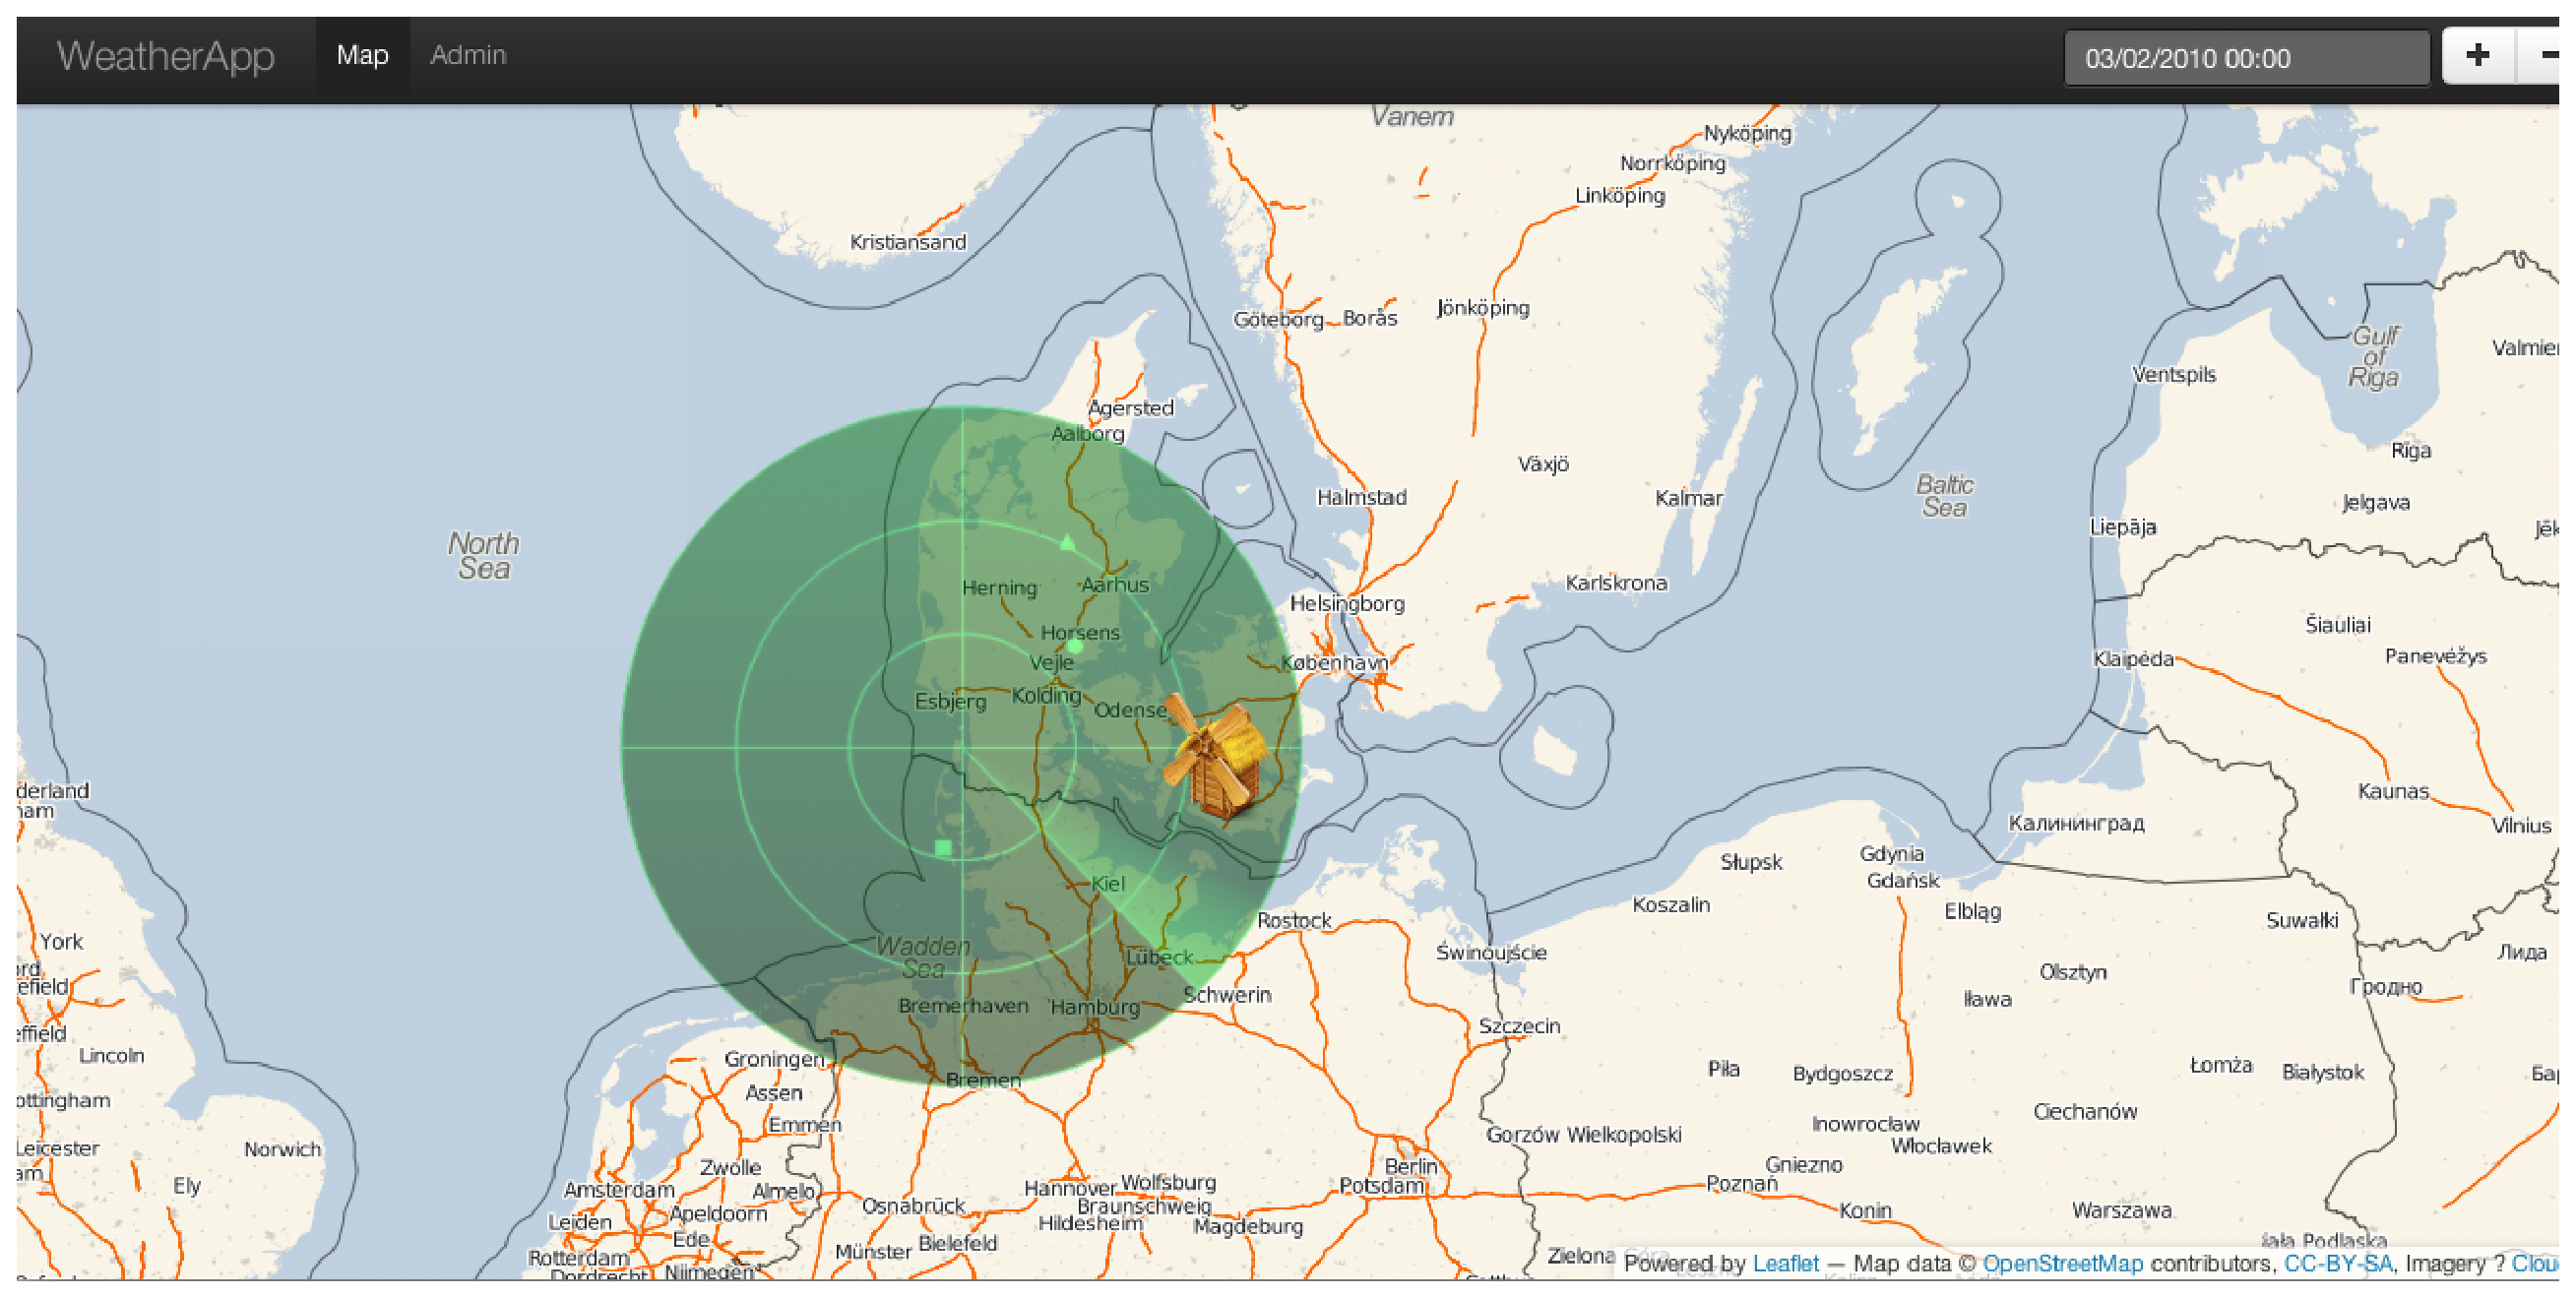
\includegraphics[scale=.3]{figure/design_map_final.eps}
   \caption{Map - final}
\end{figure}

\section{Chart}
At the beginning we had the same sidebar as on the map, but with other options. This was also replaced by a top bar like on the map.

First mockup: 
\begin{figure}[htbp]
   \centering
   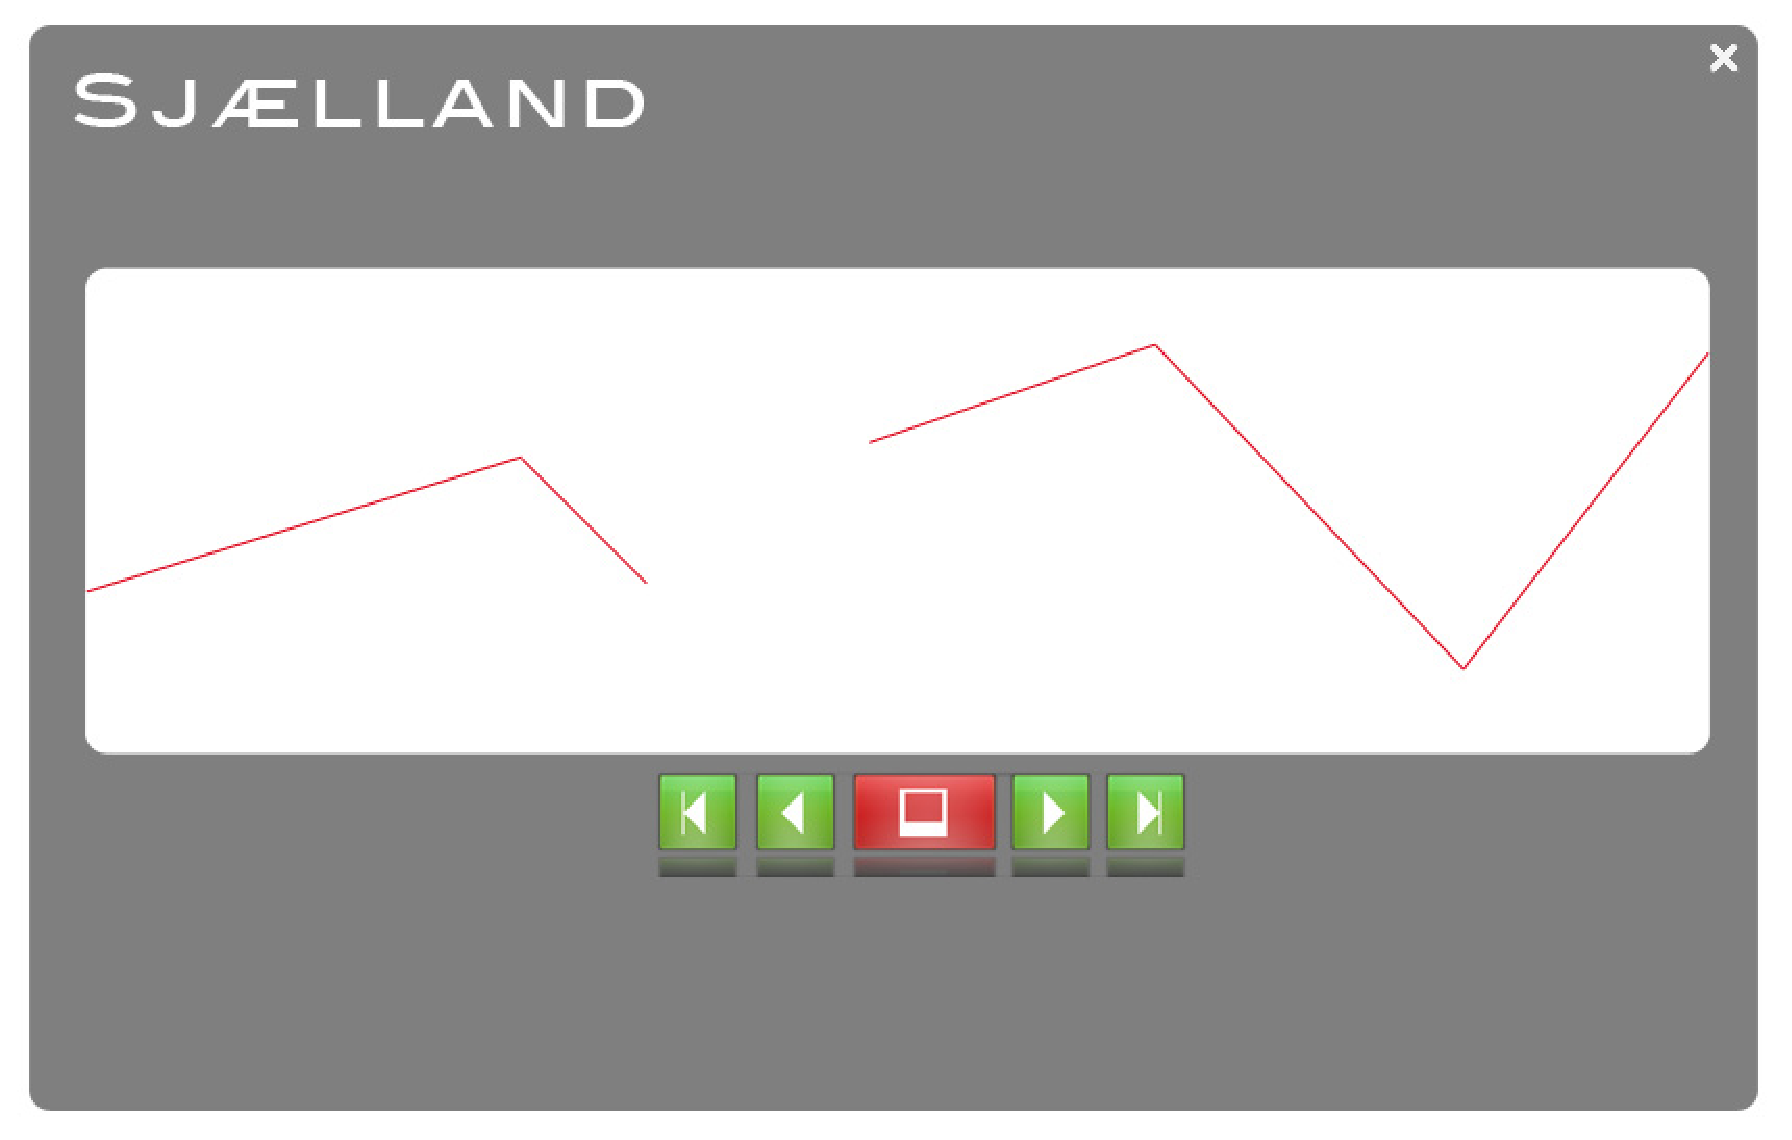
\includegraphics[scale=.3]{figure/design_chart_v1.eps}
   \caption{Chart pop up - version 1}
\end{figure}

This has, through the whole project, been determined to be a pop up on the map.
The control buttons were before 'fast backward', 'backward', 'today', 'forward' and 'fast forward', but 'today' has been replaced with a 'play' button. The 'play' button moves the chart every second, so the user can view the chart animated.

The new design have three different views '2-week', 'weekly' and 'daily view'. Control buttons adjust to the view the user has selected.

\begin{figure}[htbp]
   \centering
   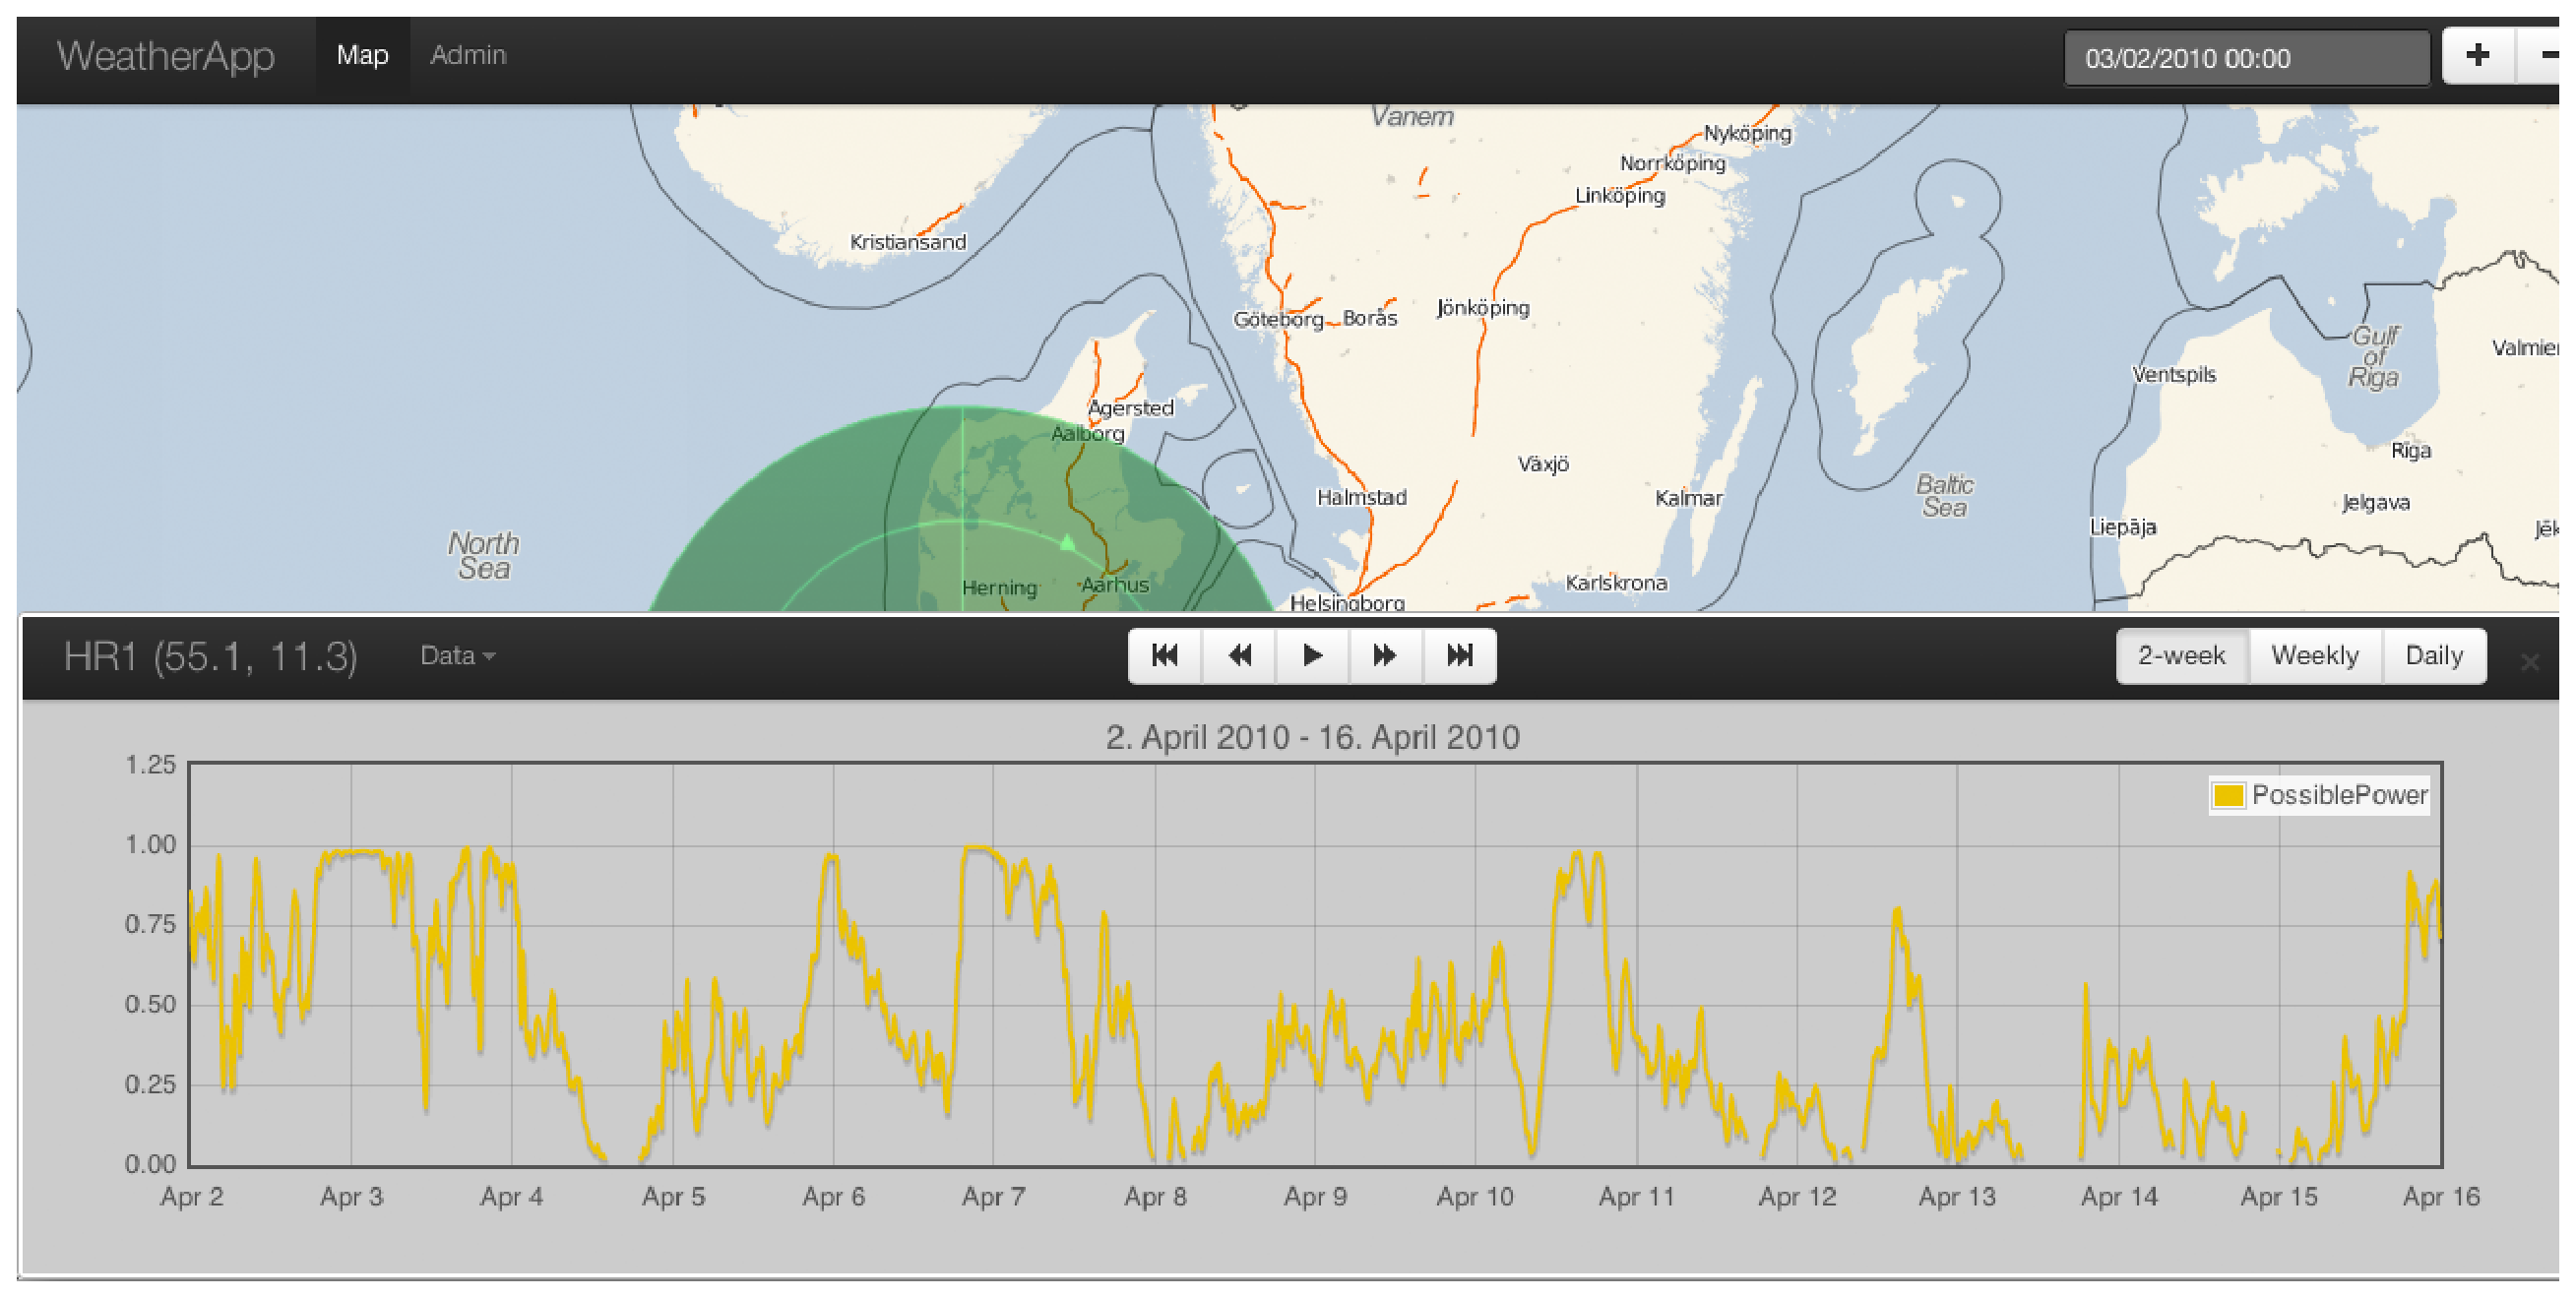
\includegraphics[scale=.3]{figure/design_chart_final.eps}
   \caption{Chart pop up - final}
\end{figure}
\chapter{Known issues}
This chapter is dedicated to highlight the known issues in the application that was not resolved due to lack of time.
\begin{itemize}
\item Due to the reset feature implemented on the radars, the windmills might do more fade in and outs than intended if the radar is clicked before an animation has finished.
This could be resolved by adding a check to see if an animation is in progress, before queuing a new one.
\item When viewing a chart, it is possible to scroll to a date that is newer than the last data of that wind farm. A check should be implemented and inform the user that the wind farm does not have any more data.
\item No versions of Internet Explorer is supported, so the application might or might not work as intended in that browser. Firefox or Google Chrome is recommended. See section \ref{sec:cross-platform} for more info.
\item If a file is uploaded with the same name as one that already exists on server, the file is skipped.
\end{itemize}

\section{Restrictions and limitations}
Under the development of the application, a few assumptions has been made, and has resulted in the following restrictions and limitations.

For the radar images to display properly, the values of \textsf{east\_uppb} and \textsf{north\_uppb} will have to be equal in the \textsf{wrk} files.

The range of the radar is calculated from \textsf{east\_uppb} and \textsf{pixel\_size}, which underlines the need for the radar image to be a perfect square.

All users have a limit on the size of the username on 50 characters and 100 characters for the email.
Also, all usernames and passwords \textbf{has} to be at least 3 characters long.

Time zone names is limited to 50 characters. Should the time zone names from zoneinfo\footnote{See section \ref{sec:application_requirements} on info about zoneinfo} exceed 50 characters, the limit can be increased by altering the database column and changing the constraint in the file model.

%%%%%%%%%%%%%%%%%%%%%%%%%%%%%%%%%%%%%%%%%%%%%%%%%%%%%%%%%%%%%%%%%%

%%%%%%%%%%%%%%%%%%%%%%%%%%%%%%%%%%%%%%%%%%
% BIBLIOGRAPHY: Build - bibtex to renew
%	\clearpage{\thispagestyle{empty}\cleardoublepage} \phantomsection 
%	\ifx\thesislanguage\danishlang
%	\addcontentsline{toc}{chapter}{Litteratur}
%	\else
%	\addcontentsline{toc}{chapter}{Bibliography}
%	\fi
%	\bibliographystyle{plainnat}
%\bibliography{bibbase}

%% Ad to Runin headings:
	\ifx\thesislanguage\danishlang
	\markboth{Litteratur}{}
	\else
	\markboth{Bibliography}{}
	\fi
%%%%%%%%%%%%%%%%%%%%%%%%%%%%%%%%%%%%%%%%%%

%%%%%%%%%%%%%%%%%%%%%%%%%%%%%%%%%%%%%%%%%%%%%%%%%%%%%%%%%%%%%%%%%%
% REFERENCE:
\clearpage{\thispagestyle{empty}\cleardoublepage} \phantomsection 
\addcontentsline{toc}{chapter}{References}
\renewcommand\bibname{References}
\bibliographystyle{plain}
\begin{thebibliography}{10}
\bibitem{VRIS}
\emph{Vejrradar informations System}.
see \texttt{Dmi\_file\_format\_description.pdf}, section `The new VRIS format'.

\bibitem{wikiBMP}
\emph{Microsoft Windows Bitmap Format}.
\url{http://en.wikipedia.org/wiki/BMP_file_format}

\bibitem{leaflet}
\emph{OpenStreetMap Leaflet documentation}.
\url{http://leaflet.cloudmade.com}

\bibitem{jquery}
\emph{jQuery documentation}.
\url{http://docs.jquery.com}

\bibitem{GPS}
\emph{Global Positioning System}.
\url{http://en.wikipedia.org/wiki/Global_Positioning_System}

\bibitem{dropbox}
\emph{Dropbox}.
\url{http://dropbox.com}

\bibitem{git}
\emph{Git}.
\url{http://github.com}
\end{thebibliography}

%%%%%%%%%%%%%%%%%%%%%%%%%%%%%%%%%%%%%%%%%%%%%%%%%%%%%%%%%%%%%%%%%%

%%%%%%%%%%%%%%%%%%%%%%%%%%%%%%%%%%%%%%%%%%%%%%%%%%%%%%%%%%%%%%%%%%
% APPENDIX:
\clearpage{\thispagestyle{empty}\cleardoublepage} \phantomsection 
	\appendix	
	\ifx\thesislanguage\danishlang
	\addcontentsline{toc}{chapter}{Appendiks}
	\else
	\addcontentsline{toc}{chapter}{Appendix}
	\fi
%\chapter{Appendix}
%\label{ap:benchmark}
%\lstinputlisting[language=c,caption={benchmark.h},label=benchmark.h]{./appendix/benchmark.h}
%\lstinputlisting[language=c,caption={benchmark.c},label=benchmark.c]{./appendix/benchmark.c}

\chapter{CSV Definition}
\label{ap:csv}
The wind farm data is of the file type csv. The file can be split up into 2 pieces.
\section{The header}
The header consists of two lines. The first line defines the latitude, longitude and the name of the wind farm from which the data originates.
The second line defines the columns, which \textbf{has} to be the same as shown in listing \ref{ap:ex:csv}.

\section{The body}
The third and following lines contains the data itself.

\section{Template}
\lstinputlisting[language=sql,caption={CSV template},label=ap:ex:csv]{./appendix/template.csv}

\chapter{Use cases}
\label{ap:usecase}
We have two types of actor:
\begin{itemize}
\item User: Ordinary person.
\item Admin: User with permission to access administration.
\end{itemize}

\section{Clicking on a radar at the map}
\textbf{Actor:} User

\textbf{Scenario:}
\begin{itemize}
\item Checks if there is data for the date
\item If images isn't generated, it will generate them real time.
\item Radar shows images over an interval.
\item \emph{One click for play/pause and doubleclick for reset.}
\item When there is no more data, the radar resets.
\end{itemize}
\textbf{Alternative scenario:} 
\begin{enumerate}
\item No data is available for that moment and a message appears.
\end{enumerate}

\section{Clicking on a wind farm at the map}
\textbf{Actor:} User

\textbf{Scenario:}
\begin{itemize}
\item Visualize data for that given wind farm.
\end{itemize}

\section{Changing view in chart for wind farm}
\textbf{Actor:} User

\textbf{Scenario:}
\begin{enumerate}
\item Changing to 2-week view.
\begin{itemize}
\item Changing chart view interval to 2 weeks.
\item Load new data for the new interval.
\end{itemize}
\item Changing to weekly view.
\begin{itemize}
\item Changing chart view interval to 1 week.
\item Load new data for the new interval.
\end{itemize}
\item Changing to daily view.
\begin{itemize}
\item Changing chart view interval to 1 day.
\item Load new data for the new interval.
\end{itemize}
\end{enumerate}

\section{Changing data to be shown}
\textbf{Actor:} User

\textbf{Scenario:}
\begin{itemize}
\item The data is shown.
\end{itemize}
\textbf{Alternative scenario}
\begin{enumerate}
\item The data is removed.
\end{enumerate}

\section{Using control buttons in chart for wind farm}
\textbf{Actor:} User

\textbf{Scenario:}
\begin{enumerate}
\item Pressing fast backward.
\begin{itemize}
\item Go two weeks back on 2-week view, one week back on weekly view and one day on daily view.
\item Loads new data.
\end{itemize}
\item Pressing backward.
\begin{itemize}
\item Go one week back on 2-week view, one day back on weekly view and one hour on daily view.
\item Loads new data.
\end{itemize}
\item Pressing play.
\begin{itemize}
\item Change to daily view and go one hour forward every second.
\item Loads new data.
\end{itemize}
\item Pressing forward.
\begin{itemize}
\item Go one week forward on 2-week view, one day forward on weekly view and one hour on daily view.
\item Loads new data.
\end{itemize}
\item Pressing fast forward.
\begin{itemize}
\item Go two weeks forward on 2-week view, one week forward on weekly view and one day on daily view.
\item Loads new data.
\end{itemize}
\end{enumerate}

\section{Upload file}
\textbf{Actor:} Admin

\textbf{Scenario:}
\begin{itemize}
\item Sign in with correct username and password.
\item Add new file (CSV, WRK, ZIP) and enter correct timezone.
\item If file is ZIP, it will decompress.
\item File is uploaded.
\item File is being parsed.
\end{itemize}
\textbf{Alternative scenario:} 
\begin{enumerate}
\item Sign in with wrong username or password.
\item Adding file that isn't correct format and get an error message.
\item Adding ZIP file, but files inside zip isn't correct. It will get an error message.
\item File exists and will not be uploaded.
\end{enumerate}

\chapter{Installation}
\label{ap:installation}
\chapter{Installation}

In the following it is implied that the chosen solutions for each step - e.g. if more than one option is possible - are compliant with the TECHNICAL REQUIREMENTS.

\begin{enumerate}
\item Download the source from \url{https://github.com/connors511/WeatherDataVisualization} in \textsf{/application}.
\item Set up a webserver to host the application, either locally or on the World Wide Web.
\item Create a database and set the connection information in \textsf{App/fuel/config/development/db.php}
\item Create the database tables. This can be done by running the following with \textsf{Oil} in command line:
\begin{lstlisting}[language=sh]
php oil g r migrate
\end{lstlisting}
\item Log in to the application with username/password: \textsf{admin/admin}.
\end{enumerate}

%%%%%%%%%%%%%%%%%%%%%%%%%%%%%%%%%%%%%%%%%%%%%%%%%%%%%%%%%%%%%%%%%%

\label{fancy:mainend} %for 'of page /x'
\clearpage{\thispagestyle{empty}\cleardoublepage}

%%%%%%%%%%%%%%%%%%%%%%%%%%%%%%%%%%%%%%%%%%
% BACK MATTER:
	\backmatter
	\ifx\thesisversion\printversion
	\makebackpage %generates the backmatter (thesislayout.sty)
	\fi
%%%%%%%%%%%%%%%%%%%%%%%%%%%%%%%%%%%%%%%%%%

\end{document}